% ==========================================================================================
% PART IV : dynamical regimes (speciation and collapse) of the masked diffusion model
% ==========================================================================================
\part{Dynamical regimes: speciation and collapse}

\section{The question}\label{sec:dr_question}
A diffusion model generates a sequence gradually. In our masked model, it starts from a fully hidden sequence
($t=1$) and reveals residues one after the other until $t=0$. Two questions can be asked about this process.
\begin{enumerate}[nosep]
\item \textbf{When does a trajectory decide which family, subfamily, or clade it will belong to?} At $t=1$ nothing is
decided. At $t=0$ the sequence is complete, so its class is fixed. Somewhere in between, the trajectory
\emph{commits}. That moment is the \textbf{speciation time} $t_S$. With a tree of classes we expect one speciation time
per level: the family is chosen first, then the subfamily, then the clade.
\item \textbf{When would a trajectory decide which \emph{training sequence} it will reproduce?} The loss we train on
has an exact minimiser, the \emph{empirical} denoiser. It only knows the $n$ training sequences, so it can only
regenerate them (memorisation). Along its trajectories there is a moment after which the final training sequence is
fixed. That is the \textbf{collapse time} $t_C$ (the ``condensation'' of the trajectory onto one data point).
\end{enumerate}
Both notions come from Biroli, Bonnaire, de Bortoli and Mézard, \emph{Dynamical regimes of diffusion models},
Nature Communications 15, 9957 (2024). They studied diffusion with \emph{Gaussian} noise in high dimension $d$ and
found three regimes in the backward (generation) process:
\begin{center}\small
\begin{tabular}{llp{9cm}}
\toprule
regime & backward time & what the trajectory knows\\
\midrule
I & $t>t_S$ & nothing: it could still end in any class\\
II & $t_C<t<t_S$ & its class, but not a specific data point (the \emph{generalisation} regime)\\
III & $t<t_C$ & the exact training point it will reproduce (only for the empirical score: memorisation)\\
\bottomrule
\end{tabular}
\end{center}
They obtained $t_S$ from the spectrum of the data covariance and $t_C$ from an entropy argument borrowed from the
statistical physics of disordered systems (the Random Energy Model).

This part does three things. First, it re-derives both results for Gaussian noise (\S\ref{sec:dr_gauss}), because
the derivations show what to transpose. Second, it transposes them to masking (\S\ref{sec:dr_mask_spec},
\S\ref{sec:dr_mask_coll}). Masking turns out to make several statements \emph{exact} rather than asymptotic. Third,
it measures both times on our trained model and on the data (\S\ref{sec:dr_results}).

%==========================================================================================
\section{The Gaussian case (the paper's setting)}\label{sec:dr_gauss}
%==========================================================================================
\subsection{Forward process}
The data $\bm x_0\in\mathbb R^d$ are noised by the Ornstein--Uhlenbeck process
$d\bm x=-\bm x\,dt+\sqrt2\,d\bm B_t$, whose solution is
\begin{equation}\label{eq:ou}
\bm x_t=e^{-t}\bm x_0+\sqrt{\Delta_t}\,\bm\xi,\qquad \Delta_t=1-e^{-2t},\qquad \bm\xi\sim\mathcal N(0,I_d).
\end{equation}
The signal shrinks as $e^{-t}$ and the noise variance grows to 1. Generation runs this backwards, from pure noise at
large $t$ to $t=0$, using the score $\nabla\log P_t$ (in practice, a network trained to approximate it).

\subsection{Speciation: two Gaussian classes}\label{sec:dr_gauss_spec}
Take two equally likely classes, $\bm x_0=\pm\bm m+\sigma\bm z$ with $\bm z\sim\mathcal N(0,I_d)$. By
\eqref{eq:ou}, given the class, $\bm x_t$ is Gaussian with mean $\pm e^{-t}\bm m$ and variance
$\Gamma_t=\sigma^2e^{-2t}+\Delta_t$ in every direction. So $P_t$ is a mixture of two Gaussians.

\paragraph{The class posterior.} By Bayes' rule, the log-odds of class $+$ against class $-$ given $\bm x_t$ is the
difference of the two Gaussian exponents:
\[
\Lambda(\bm x_t)=\log\frac{P(+\mid\bm x_t)}{P(-\mid\bm x_t)}
=\frac{\|\bm x_t+e^{-t}\bm m\|^2-\|\bm x_t-e^{-t}\bm m\|^2}{2\Gamma_t}=\frac{2e^{-t}\,\bm m\cdot\bm x_t}{\Gamma_t}.
\]
(The $\|\bm x_t\|^2$ and $\|\bm m\|^2$ terms cancel.) Now let $\bm x_t$ come from class $+$. Then
$\bm m\cdot\bm x_t=e^{-t}\|\bm m\|^2+\sqrt{\Gamma_t}\,\|\bm m\|\,g$ with $g\sim\mathcal N(0,1)$, since the projection of
isotropic noise of variance $\Gamma_t$ on the direction of $\bm m$ has variance $\Gamma_t\|\bm m\|^2$. Therefore
\begin{equation}\label{eq:llr_gauss}
\Lambda=\mu_t+\sqrt{2\mu_t}\,g,\qquad \mu_t=\frac{2\|\bm m\|^2e^{-2t}}{\Gamma_t}.
\end{equation}
The log-odds is Gaussian with mean $\mu_t$ and variance $4\|\bm m\|^2e^{-2t}/\Gamma_t=2\mu_t$. This mean/variance
relation is not an accident. A log-likelihood ratio must satisfy $\E_-[e^{\Lambda}]=1$ (the likelihood ratio averages
to 1 under the other class), and for a Gaussian $\Lambda$ this forces variance $=2\times$mean. We call $\mu_t$ the
\textbf{class signal-to-noise ratio}.

\paragraph{The cloning experiment.} The paper measures commitment like this: stop a backward trajectory at time $t$,
make two copies (``clones''), and continue both independently to $t=0$. Given $\bm x_t$, each clone ends in class
$+$ with probability $p=P(+\mid\bm x_t)$. So the two clones end in the same class with probability $p^2+(1-p)^2$.
Averaging over $\bm x_t$:
\begin{equation}\label{eq:phi_def}
\phi(t)=\E_{\bm x_t}\Big[\sum_cP(c\mid\bm x_t)^2\Big].
\end{equation}
$\phi$ goes from $\sum_c\pi_c^2=1/2$ (nothing decided) to 1 (decided). Normalise it to run from 0 to 1:
$\psi=(\phi-\phi_0)/(1-\phi_0)$. For two classes, $p=1/(1+e^{-\Lambda})$ gives
$p^2+(1-p)^2=\tfrac12\big(1+(2p-1)^2\big)=\tfrac12\big(1+\tanh^2(\Lambda/2)\big)$. Hence
\begin{equation}\label{eq:psi_universal}
\boxed{\psi=\E\big[\tanh^2(\Lambda/2)\big]=:\Psi(\mu),\qquad \Lambda\sim\mathcal N(\mu,2\mu).}
\end{equation}
The commitment is a \emph{universal} function of the single number $\mu$. It is 0 at $\mu=0$, tends to 1 as
$\mu\to\infty$, and crosses $1/2$ at $\mu^\star=1.70$ (computed numerically).

\paragraph{The speciation time.} Define $t_S$ by $\psi(t_S)=1/2$, i.e.\ $\mu_{t_S}=\mu^\star$. Speciation happens when
the noise is already large, so $\Gamma_t\approx1$, and
\begin{equation}\label{eq:ts_gauss}
2\|\bm m\|^2e^{-2t_S}=\mu^\star\ \Longrightarrow\ t_S=\tfrac12\log\|\bm m\|^2+\tfrac12\log(2/\mu^\star)\approx\tfrac12\log\Lambda_{\max}.
\end{equation}
The covariance of the data is $\bm m\bm m^\top+\sigma^2I$, whose largest eigenvalue is
$\Lambda_{\max}=\|\bm m\|^2+\sigma^2\approx\|\bm m\|^2$. In high dimension $\Lambda_{\max}$ grows with $d$, and the
$O(1)$ constant is negligible. That gives the paper's formula $t_S=\tfrac12\log\Lambda_{\max}$.

\paragraph{The same time, seen as a symmetry breaking.} The paper derives $t_S$ from the shape of the potential
$U_t=-\log P_t$, which drives the backward dynamics. Along the direction of $\bm m$ at the midpoint $\bm x=0$,
differentiating the two-Gaussian mixture twice gives a curvature
$\partial^2\log P_t=-1/\Gamma_t+e^{-2t}\|\bm m\|^2/\Gamma_t^2$. For large $t$ it is negative: a single well, and
the trajectory is not attracted to either class. It changes sign when $e^{-2t}\|\bm m\|^2=\Gamma_t\approx1$, the same
$t_S$ up to the $O(1)$ constant. Below $t_S$ the potential has two wells and each trajectory falls into one: the
symmetry between classes is broken. \texttt{test\_17} simulates this two-Gaussian system ($d=50$,
$\|\bm m\|^2=400$). It checks that the measured commitment follows $\Psi(\mu_t)$ at every $t$ and crosses 1/2 at
$\tfrac12\log(2\|\bm m\|^2/\mu^\star)$ (Fig.~\ref{fig:dr_tests}, left).

\subsection{Collapse: the empirical score and the Random Energy Model}\label{sec:dr_gauss_coll}
Now suppose the model has learned the score of the \emph{empirical} distribution of $n$ training points
$\bm a_1,\dots,\bm a_n$ (the exact minimiser of the denoising loss on the training set). The noised empirical
distribution is a mixture of $n$ small Gaussians:
\[
P^e_t(\bm x)=\frac1n\sum_{\mu=1}^n\mathcal N\big(\bm x;\,e^{-t}\bm a_\mu,\,\Delta_tI\big).
\]
The backward process with this score reproduces $P^e_t$ at every time. At $t=0$ it therefore returns a training
point. A trajectory that ends at $\bm a_1$ is, at time $t$, $\bm x_t=e^{-t}\bm a_1+\sqrt{\Delta_t}\bm\xi$. How strongly
does it already ``belong'' to $\bm a_1$? Compare the Gaussian weight of $\bm a_1$ with the total weight of all the
others:
\[
w_1=\mathcal N(\bm x_t;e^{-t}\bm a_1,\Delta_t)\approx(2\pi e\Delta_t)^{-d/2},
\qquad \sum_{\mu\ge2}w_\mu\approx(n-1)\,\E_{\bm a}\big[\mathcal N(\bm x_t;e^{-t}\bm a,\Delta_t)\big]=(n-1)P_t(\bm x_t).
\]
The first uses $\|\bm\xi\|^2\approx d$. The second is the law of large numbers: the other training points are
independent draws from the true $P_0$, and averaging the Gaussian kernel over $P_0$ gives the true noised density
$P_t$. With $-\frac1d\log P_t(\bm x_t)\approx s(t)$, the entropy per dimension of $P_t$:
\begin{equation}\label{eq:collapse_gauss}
\frac{\sum_{\mu\ge2}w_\mu}{w_1}\approx n\,e^{-d\,f(t)},\qquad f(t)=s(t)-\tfrac12\log(2\pi e\Delta_t).
\end{equation}
$f(t)$ is the \textbf{excess entropy}: the entropy of $P_t$ minus the entropy of the noise alone. It measures how many
distinguishable ``noise balls'' the data occupy. While $n e^{-d f(t)}\gg1$, the other points dominate: the trajectory
is surrounded by many training points and has not chosen. When $n e^{-d f(t)}\ll1$, $\bm a_1$ dominates and the
trajectory has collapsed. The collapse time solves
\begin{equation}\label{eq:tc_gauss}
\boxed{f(t_C)=\frac{\log n}{d}.}
\end{equation}
The law-of-large-numbers step fails exactly at $t_C$. Below it, the sum over $\mu$ is dominated by a single term, as
the partition function of the Random Energy Model is dominated by its lowest energy levels below the glass
(``condensation'') transition. This is why the paper borrows REM methods, and why the typical (``quenched'') and the
average (``annealed'') values of the sum differ.

\paragraph{The picture.} Speciation depends on the class structure (the top eigenvalue), not on $n$. Collapse
depends on $n$: more data pushes $t_C$ to smaller $t$, and for $\log n\propto d$ the two are well separated. A
network trained on the same data \emph{generalises} if it does not reproduce the empirical score below $t_C$.

%==========================================================================================
\section{From Gaussian noise to masking}\label{sec:dr_mask}
%==========================================================================================
\subsection{Time, revealed sites, and what the noise does}
In our model (Part~III) the noise is masking. At time $t$ every site is hidden independently with probability $t$,
so the number of \textbf{revealed sites} is $k\sim\mathrm{Binomial}(L,1-t)$, with mean $L(1-t)$. Given $k$, the set
$U$ of revealed sites is a uniformly random $k$-subset, \emph{independent of the sequence}. Everything below is
therefore computed at fixed $k$ and converted to $t$ at the end:
\begin{equation}\label{eq:k_to_t}
\langle f\rangle(t)=\sum_{k=0}^L\binom Lk(1-t)^kt^{L-k}\,f_k .
\end{equation}
Because the mask is independent of the data, the posterior over the clean sequence is just the data distribution
conditioned on the revealed residues:
\begin{equation}\label{eq:mask_posterior}
P(\bm x_0\mid\bm x_t)=P(\bm x_0\mid \bm x_U)\propto P(\bm x_0)\,\one[\bm x_{0,U}=\bm x_U].
\end{equation}
Two differences with Gaussian noise matter.
\begin{itemize}[nosep]
\item A revealed residue is \emph{exact}, and a hidden one carries \emph{no} information. There is no partial
information per site.
\item The reverse direction is ``$k$ grows'': $k=0$ at $t=1$ (start of generation) and $k=L$ at $t=0$. A
\emph{large} speciation time $t_S$ means the class is decided \emph{early}, after few revealed sites.
\end{itemize}

\subsection{Speciation for masking}\label{sec:dr_mask_spec}
\paragraph{Cloning, exactly.} Let $y(\bm x)$ be any deterministic label of complete sequences, for instance the clade
assigned by a classifier. From a partially revealed $\bm x_t$, complete it $C$ times independently with the denoiser
(``clones''). With the exact denoiser, each completion is an independent draw from $P(\bm x_0\mid\bm x_U)$, so
\begin{prop}[clone agreement]\label{prop:clone}
With the exact denoiser, (i) two clones get the same label with probability
$\phi_k=\E\big[\sum_yP(y\mid\bm x_U)^2\big]$; (ii) a clone gets the \emph{same label as the original sequence} with the
same probability $\phi_k$.
\end{prop}
\emph{Proof.} (i) Given $\bm x_U$ the clones are independent with label distribution $P(y\mid\bm x_U)$, so they agree
with probability $\sum_yP(y\mid\bm x_U)^2$; then average. (ii) The original $\bm x_0$ is itself a draw from
$P(\bm x_0\mid\bm x_U)$, independent of the clones given $\bm x_U$, so the same computation applies. $\square$

Part (ii) gives a consistency check on a \emph{trained} network. If its clones agree with each other more (or less)
than with the original, its conditional distributions are wrong.

\paragraph{The network's own trajectories.} The exact continuous-time sampler (Part~III) reveals sites in a uniformly
random order at independent random times, both drawn independently of the residues. So at any time $t$ of a
generated trajectory, $\bm x_t$ is the final sample with a random, sequence-independent set of sites hidden.
\emph{Masking the network's samples therefore gives exactly its trajectories at time $t$.} We use two starting
ensembles: (A) masked \textbf{held-out true} sequences, which probe the network on the true $\bm x_t$; and (B) masked
\textbf{network samples}, which are its own trajectories.

\paragraph{Theory: the class log-odds for masking.} Let each class $c$ be summarised by its site frequencies
$f_{c,i}(a)$ (the \emph{profile} approximation, which ignores couplings). Given the revealed residues, Bayes' rule
gives
\begin{equation}\label{eq:profile_post}
\log P(c\mid\bm x_U)=\log\pi_c+\sum_{i\in U}\log f_{c,i}(x_i)-\text{normaliser}.
\end{equation}
Between two classes $c,c'$ the log-odds is a sum over revealed sites,
$\Lambda=\sum_{i\in U}\log\frac{f_{c,i}(x_i)}{f_{c',i}(x_i)}$. For $\bm x$ from $c$, each site contributes on average
$\mathrm{KL}(f_{c,i}\|f_{c',i})$, and each site is revealed with probability $k/L$. Hence
\begin{equation}\label{eq:mu_mask}
\E\Lambda=\mu_k=\frac kL\,D,\qquad D=\sum_{i=1}^L\mathrm{KL}(f_{c,i}\,\|\,f_{c',i}).
\end{equation}
\emph{Variance.} Write $f_{c',i}=f_{c,i}(1+\varepsilon_i)$ with small $\varepsilon_i$. The per-site log-ratio
$r_i=-\log(1+\varepsilon_i)$ has mean $\mathrm{KL}_i\approx\frac12\E\varepsilon_i^2$ and variance
$\approx\E\varepsilon_i^2=2\,\mathrm{KL}_i$. Summing independent sites gives $\mathrm{Var}\,\Lambda\approx2\mu_k$: the
same ``variance $=2\times$mean'' law as \eqref{eq:llr_gauss}. When many weakly informative sites are revealed,
$\Lambda$ is approximately Gaussian, and the commitment follows the \emph{same universal curve} $\Psi(\mu)$ of
\eqref{eq:psi_universal}, with the time dependence
\begin{equation}\label{eq:snr_compare}
\text{Gaussian noise: }\mu_t\approx2\Lambda_{\max}e^{-2t},\qquad\qquad\text{masking: }\mu_t=(1-t)\,D.
\end{equation}
Setting $\mu=\mu^\star$:
\begin{equation}\label{eq:ts_mask}
\boxed{k_S=\frac{L\,\mu^\star}{D},\qquad t_S=1-\frac{\mu^\star}{D}.}
\end{equation}
The role of the top covariance eigenvalue is played by $D$, the total information that a fully revealed sequence
carries about its class relative to a sibling class. For our tree, the siblings of each level are the classes that
share the same parent. The hierarchy then predicts a \textbf{cascade of speciations}:
$D_{\rm family}>D_{\rm subfamily}>D_{\rm clade}$, so families are decided first, then subfamilies, then clades. With
the measured profiles (\S\ref{sec:dr_results}) $D=64,\,23,\,10$ nats, so
$k_S\approx1.6,\,4.4,\,9.8$ revealed sites.

Two caveats. (1) With few revealed sites, $\Lambda$ is a sum of a few terms and is not Gaussian. We therefore also
compute the \emph{profile-Bayes} commitment exactly, by Monte Carlo over true sequences and random masks with
\eqref{eq:profile_post}. (2) Couplings carry extra class information (in our tree, parent-to-child perturbations
also change $J$), and pairs of revealed residues can reveal it. The true commitment can therefore rise earlier than
the profile prediction.

\paragraph{A data-only estimate.} Before collapse, many training sequences agree exactly with $\bm x_U$. Their class
labels give a model-free estimate of $P(c\mid\bm x_U)$: the fraction of matching training sequences in class $c$. We
use it only when at least 20 sequences match. It is exact as $n\to\infty$ and, by construction, is available only
in regime I and early regime II. This is where the two times meet.

\subsection{Collapse for masking}\label{sec:dr_mask_coll}
\paragraph{The empirical denoiser.} Put the uniform distribution on the $n$ training sequences into
\eqref{eq:mask_posterior}. The posterior is uniform over the $N$ training sequences that agree with $\bm x_t$ on every
revealed site:
\begin{equation}\label{eq:emp_post}
P^e(\bm x_0=\bm a_\mu\mid\bm x_t)=\frac{\one[\bm a_{\mu,U}=\bm x_U]}{N(\bm x_t)},\qquad
N(\bm x_t)=\sum_{\mu=1}^n\one[\bm a_{\mu,U}=\bm x_U].
\end{equation}
Applying Proposition~\ref{prop:clone} with the label ``which training sequence'': \textbf{two clones end at the same
training sequence with probability $\E[1/N]$.} This is the collapse analogue of $\phi$. It is $1/n$ at $k=0$ and 1
once $N=1$.

\paragraph{How many training sequences match?} Follow a trajectory of the empirical denoiser that ends at training
sequence $\bm a_1$ (it is planted on $\bm a_1$). The planted sequence always matches. Each of the $n-1$ others is an
independent draw from the true distribution and matches with probability $P(\bm a_{1,U})$, the true probability of the
revealed residues. So, exactly,
\[
N=1+\mathrm{Binomial}\big(n-1,\ P(\bm a_{1,U})\big)\approx1+\mathrm{Poisson}(\lambda),\qquad \lambda=(n-1)\,P(\bm a_{1,U}).
\]
For $M\sim\mathrm{Poisson}(\lambda)$:
$\E\big[\tfrac1{1+M}\big]=\sum_m\frac{e^{-\lambda}\lambda^m}{(m+1)!}=\frac{e^{-\lambda}}\lambda\sum_{m\ge1}\frac{\lambda^m}{m!}
=\frac{1-e^{-\lambda}}{\lambda}$. Therefore
\begin{equation}\label{eq:collapse_mask}
\boxed{\E[1/N]=\E_{\bm a,U}\Big[\frac{1-e^{-\lambda}}{\lambda}\Big],\qquad \lambda=(n-1)P(\bm a_U).}
\end{equation}
This is the \textbf{quenched} prediction: the average is taken over the actual fluctuating $\lambda$. It crosses $1/2$
at $\lambda=1.59$. For typical $\bm a$, $-\log P(\bm a_U)\approx H(k)$, the entropy of $k$ revealed residues
(asymptotic equipartition), so collapse happens when
\begin{equation}\label{eq:tc_mask}
\boxed{H(k_C)=\log n.}
\end{equation}
This is \eqref{eq:tc_gauss} for masking. The ``excess entropy'' is simply $H(k)$, the entropy of the revealed
residues. A revealed residue carries no noise, so the ``noise ball'' around a data point contains exactly one
sequence (entropy 0), and nothing needs to be subtracted.

\paragraph{The annealed prediction, and why it is wrong.} Averaging $\lambda$ first replaces $P(\bm a_U)$ by its mean
$\E_{\bm a}P(\bm a_U)=\sum_{\bm x_U}P(\bm x_U)^2$. This is the probability that two independent sequences agree on the
$k$ revealed sites, and it can be read off pairwise Hamming distances. A pair at distance $D_{ab}$ agrees on a random
$k$-subset iff none of its $D_{ab}$ mismatches is revealed:
\begin{equation}\label{eq:collision}
\E_{\bm a}P(\bm a_U)=\E_{\text{pairs}}\Big[\binom{L-D_{ab}}{k}\Big/\binom Lk\Big]=e^{-H_2(k)},
\end{equation}
where $H_2$ is the Rényi-2 (collision) entropy. Since $H_2\le H$ (Jensen), the annealed average counts \emph{more}
matches than a typical trajectory sees. It is dominated by rare close pairs (same clade, small $D_{ab}$), exactly as
the annealed REM partition function is dominated by rare low energies. So it predicts a \emph{later} collapse (larger
$k_C$). The quenched formula \eqref{eq:collapse_mask} is the correct one; we show both.

\paragraph{Getting $H(k)$ from the network.} Let $i_1,i_2,\dots$ be the reveal order. By the chain rule,
\[
\log P(\bm x_{U_k})=\sum_{j=0}^{k-1}\log P\big(x_{i_{j+1}}\mid\bm x_{U_j}\big).
\]
The trained denoiser provides every factor,
so one pass of $L$ network calls gives $\log P_\theta(\bm x_{U_k})$ for all $k$. Averaged over sequences and orders,
$-\log P_\theta(\bm x_{U_L})$ is the NELBO of Part~III. Because the network's conditionals are close to the truth
(TV 0.10, Part~III), $P_\theta$ is a good stand-in for $P$ in \eqref{eq:collapse_mask}. It slightly overestimates
entropies, since a cross-entropy is at least the entropy.

\paragraph{Collapse versus $n$: the phase diagram.} $\log n$ enters only through \eqref{eq:collapse_mask}. So from
the same $P_\theta(\bm x_U)$ we can predict $k_C(n)$ for any $n$, and measure it directly on training subsets of size
$n$. Speciation at level $\ell$ happens before collapse (regimes cleanly separated) only if
\[
H(k_S^\ell)<\log n\iff n>n^\star_\ell=e^{H(k_S^\ell)}.
\]
For a small training set, the empirical denoiser picks a training sequence before it has even decided the clade, so
the clade is inherited from the memorised sequence.

\paragraph{Memorisation of the trained network.} The empirical denoiser is the \emph{exact minimiser} of the training
loss. Its NELBO on training data is $\log n/L$ nats per site, and it is infinite on new data. A network that reached it
would reproduce training sequences: along its trajectories, $\bm x_t$ would always match at least one training
sequence ($N\ge1$), as for planted trajectories. A generalising network produces trajectories that stop matching
the training set, like held-out true sequences do. We compare $P(N\ge1)$ along three kinds of trajectories:
planted on training sequences (always 1), held-out sequences, and the network's own samples.

%==========================================================================================
\section{Implementation}\label{sec:dr_impl}
%==========================================================================================
\begin{center}\footnotesize
\begin{tabular}{p{4.6cm}p{9.6cm}}
\toprule
function (\texttt{src/psg/regimes.py}) & what it computes\\
\midrule
\texttt{random\_orders}, \texttt{reveal\_first\_k} & a uniformly random reveal order per sequence; $\bm x_t$ with the first $k$ sites of the order revealed\\
\texttt{complete} & $C$ independent completions of each $\bm x_t$: masked sites revealed one at a time in random order,
each drawn from the denoiser at $t=$ current fraction masked (the exact reverse process for a $t$-independent denoiser, Part~III)\\
\texttt{pair\_agreement} & fraction of the $C(C-1)/2$ clone pairs with equal labels, per starting point\\
\texttt{profile\_log\_posterior} & \eqref{eq:profile_post}\\
\texttt{gaussian\_llr\_commitment}, \texttt{solve\_mu\_star} & $\Psi(\mu)$ of \eqref{eq:psi_universal} by Gauss--Hermite quadrature; $\mu^\star$ by bisection\\
\texttt{sibling\_kl} & $D$ of \eqref{eq:mu_mask}, averaged over ordered sibling pairs\\
\texttt{consistent\_counts} & $N(\bm x_t)$ of \eqref{eq:emp_post} on the GPU, optionally split by class\\
\texttt{poisson\_commitment} & $(1-e^{-\lambda})/\lambda$\\
\texttt{subset\_agreement} & the collision probability \eqref{eq:collision}\\
\texttt{revealed\_log\_prob} & $\log P_\theta(\bm x_{U_k})$ for all $k$ by the chain rule ($L$ network calls)\\
\texttt{to\_time}, \texttt{crossing} & the binomial average \eqref{eq:k_to_t}; the level-crossing point by linear interpolation\\
\texttt{pseudo\_loglik\_scores\_torch} (in \texttt{evaluation.py}) & the clade classifier of Part~III on the GPU: all local fields at once as
$h+\mathrm{onehot}(\bm x)\,J_{\rm flat}^\top$\\
\bottomrule
\end{tabular}
\end{center}

\paragraph{The script \texttt{s13\_dynamical\_regimes.py}.}
\begin{enumerate}[nosep]
\item \emph{Labels.} Every completed sequence is assigned the clade with the largest pseudo-log-likelihood under the 18
true clade models (as in Part~III). Its family and subfamily follow from the clade. On labelled test sequences
the classifier is right for 100\% of families, 99.4\% of subfamilies and 91.5\% of clades. Commitment is therefore
measured for classifier-defined classes, which is legitimate because Proposition~\ref{prop:clone} holds for any
deterministic label.
\item \emph{Cloning.} 1000 starting sequences per ensemble ((A) held-out test sequences, (B) fresh network samples),
each with its own random reveal order. For every $k\in\{0,\dots,20,24,28,34,40,50,60\}$: reveal the first $k$
sites and complete 8 clones. That is 8000 completions per $k$ and $\approx2\times10^5$ per ensemble. We record
$\phi_k$, its standard error, and the agreement with the original's label.
\item \emph{Theory.} Profiles per class from the training set (pseudo-count $10^{-3}$). The profile-Bayes commitment on
5000 test sequences for every $k$; the sibling divergences $D$; the Gaussian prediction \eqref{eq:ts_mask}.
\item \emph{Counting.} For every $k$, $N$ for (A), for (B), and for 1000 trajectories planted on training sequences
(C), against all $n=144\,000$ training sequences. This gives the data-only speciation estimate (for (A), when
$N\ge20$), the measured collapse $\E[1/N]$ (C), and the memorisation check $P(N\ge1)$ for (A), (B), (C).
\item \emph{Collapse theory.} $\log P_\theta(\bm x_{U_k})$ for (A) and (C); $H(k)$; the quenched prediction
\eqref{eq:collapse_mask}; the annealed prediction from $4\times10^5$ random training pairs; the phase diagram
(measured on subsets $n=10^2,10^3,10^4,144\,000$, predicted for $n$ up to $10^{60}$).
\item \emph{Single trajectories.} Six network trajectories; at each $k\le20$, 64 clones, giving the fraction that
ends in the trajectory's final family or clade, a direct picture of commitment.
\end{enumerate}
The time $t_S$ (or $t_C$) is where the binomially averaged curve \eqref{eq:k_to_t} crosses $1/2$. The number of
revealed sites $k_S$ (or $k_C$) is where the fixed-$k$ curve crosses $1/2$.

\section{Tests of Part IV}\label{sec:dr_tests}
\begin{center}\footnotesize
\begin{tabular}{p{5.2cm}p{9cm}}
\toprule
test (\texttt{tests/test\_17\_regimes.py}) & what it checks\\
\midrule
\texttt{pair\_agreement}, normalisation & by hand: labels $(0,0,0,0)\to1$, $(0,1,0,1)\to2/6$\\
\texttt{to\_time}, \texttt{crossing} & $f(k)=k$ averages to $L(1-t)$ exactly; a crossing by hand\\
random orders & each row is a permutation; each site is revealed with probability $k/L$\\
profile posterior & one site, profiles $(0.9,0.1)$ vs $(0.1,0.9)$: posterior 0.9/0.1, and the prior when masked\\
\texttt{consistent\_counts} & by hand on 3 training sequences, total and per class\\
collision, Poisson & $\binom{L-D}k/\binom Lk$ by hand and by Monte Carlo; $\E[1/(1+M)]$ for $M\sim$ Poisson by simulation\\
GPU classifier & equal to the numpy pseudo-log-likelihood\\
Gaussian speciation & two Gaussians in $d=50$: measured commitment $=\Psi(\mu_t)$ (to 0.01) at all $t$; $t_S=\frac12\log(2\|\bm m\|^2/\mu^\star)$; $\Psi(0)=0$, $\Psi(\mu^\star)=1/2$\\
cloning, exact denoiser & two-class profile mixture ($L=4$, $q=3$) enumerated: clone agreement and clone-vs-original agreement equal the exact $\E\sum_yP(y\mid\bm x_U)^2$ for every $k$ (to 0.02); revealed sites are never changed\\
chain rule & $\log P(\bm x_{U_k})$ from the exact denoiser equals the enumerated marginal, for every $k$\\
empirical collapse & empirical denoiser on 12 training sequences: clones land on the same training sequence with probability $\E[1/N]$ for every $k$; $1/n$ at $k=0$, 1 at $k=L$\\
pipeline & the whole of \texttt{s13} on a tiny tree with a tiny trained model: $\psi=0$ at $k=0$ and 1 at $k=L$, planted trajectories always match, all figures written\\
\bottomrule
\end{tabular}
\end{center}

\begin{figure}[H]
\centering
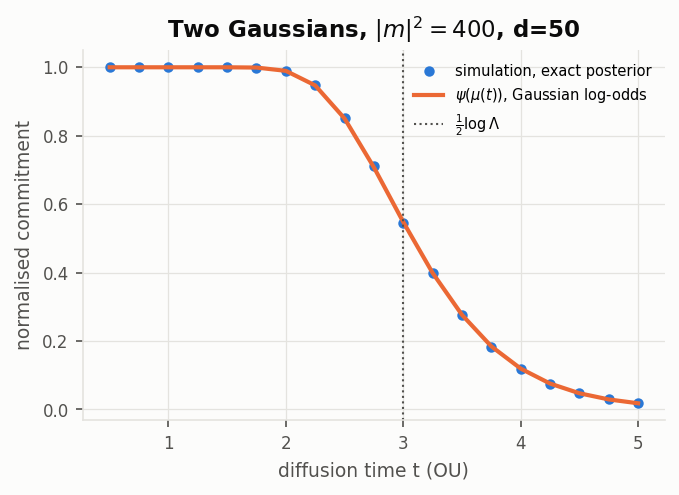
\includegraphics[width=0.32\textwidth]{tests/test_17_regimes/test_gaussian_mixture_speciation/gaussian_speciation.png}\hfill
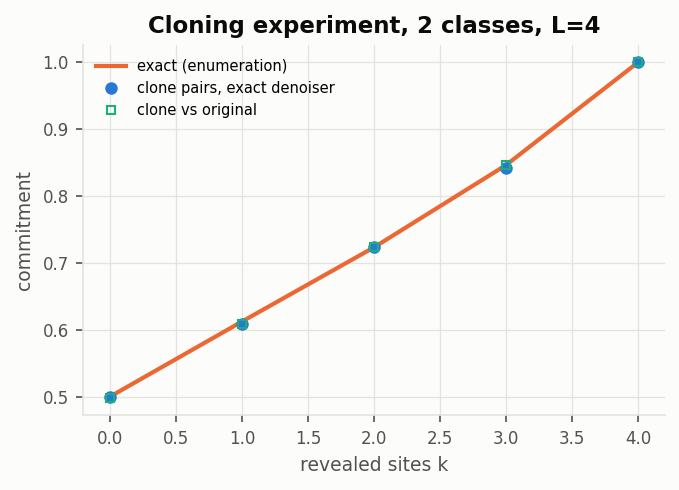
\includegraphics[width=0.32\textwidth]{tests/test_17_regimes/test_cloning_with_exact_denoiser_gives_exact_commitment/cloning_exact.png}\hfill
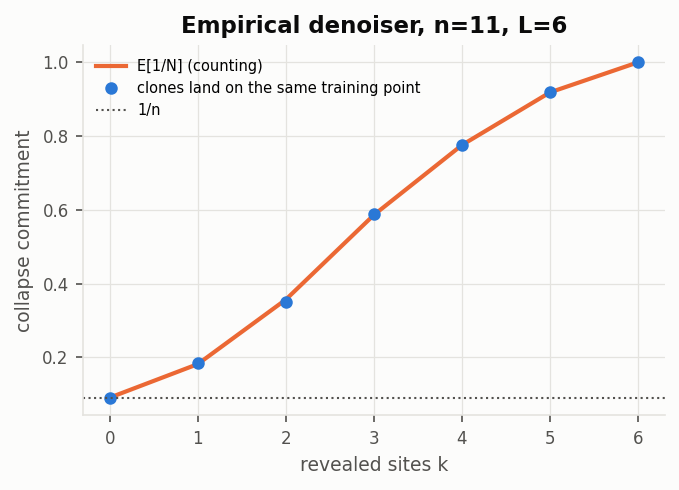
\includegraphics[width=0.32\textwidth]{tests/test_17_regimes/test_empirical_denoiser_collapse_is_one_over_n/empirical_collapse.png}
\caption{Tests of the measurement tools. Left: two Gaussian classes under OU noise; the commitment follows the
universal curve $\Psi(\mu_t)$ and crosses $1/2$ near $\frac12\log\Lambda_{\max}$. Middle: cloning with the exact denoiser
reproduces the exact commitment. Right: with the empirical denoiser, the probability that two clones land on the same
training sequence is $\E[1/N]$.}
\label{fig:dr_tests}
\end{figure}
